\documentclass{pracjourn}[2006/02/20]

\usepackage{graphics}

% Uncomment these lines when using pdfscreen
%\usepackage[screen,panelright,paneltoc]{pdfscreen}
%\margins{0.75in}{0.75in}{0.75in}{0.75in}
%\screensize{6.25in}{8in}

%%% Revision control
\TPJissue{2011}{1}
\TPJrevision{2011}{09}{10}
%%%

\title{Integrating LaTeX and Moodle Questionnaires}

\author{L. Garcia-Forte, C. Leon-Hernandez and C. Rodriguez-Leon}

\abstract{
The manufacturing of teaching material conveys the generation
of both static (unreactive) data-documents 
and dynamic (reactive) program-documents
based on different technologies.
Teaching a subject often implies the maintenance
of a large number of both types of 
documents, usually written in a variety of languages
and stored in diferent formats.
Ergo a natural goal for the lecturer is to minimize the amount of work invested 
during the development and maintenance of the material.
There are acceptable 
solutions regarding the transformation between 
formats with the same kind of reactivity.
This work discusses the problem of integrating Moodle 
(a Open Source Learning Management System)
and \LaTeX{} (a  document preparation system),
proposes a methodology to pursuit this goal and presents a tool to assist 
in the translation of Moodle Quiz documents to \LaTeX{}.}

\email {lgforte@ull.es, cleon@ull.es, casiano@ull.es}
\website{http://nereida.deioc.ull.es} 
\address{Dpto. Estad\'{\i}stica, I.O. y Computaci\'on \\
       Universidad de La Laguna \\
       Tenerife, Spain }

\license{Copyright \textcopyright\ 2010.\\
  Permission is granted to distribute verbatim or modified\\
  copies of this document provided this notice remains intact.}
%%%

%%% Defining more metadata:
%\addinfospace{1ex}
%\addinfo[\color{blue}\scshape]{Hobby}
%\hobby{Sleeping in.}
%%%

%%% Changing the hyperlink colour:
\definecolor{linkcolour}{rgb}{0.7,0.2,0.2}
%%%


\begin{document}
\maketitle


%\hyphenation{a-ssist de-ve-lo-ped e-xams su-pport o-ppor-tu-ni-ties
%             gi-ving bet-ween ge-ne-ra-te Do-cu-ment Pre-pa-ra-tion
%             pro-blem for-mi-da-ble Moo-dle im-por-ting ques-tions
%             com-pre-hen-si-ve ex-port ques-tio-nai-ries
%             Mark-up lan-gua-ges Hy-per-text hy-per-me-dia
%             Pre-pa-ring Main-tain-ing Ques-tio-nnai-res
%             par-ti-cu-lar-ly de-li-mi-ters
%             Hy-per-text hy-per-me-dia
%             }

%%%%%%%%%%%%%%%%%%%%%%%%%%%%%%%%%%%%%%%%%%%%%%%%%%%%%%%%%%%%%%%%%%%%%%%%%%%%%%%%%%%%%%%%%
\section{Introduction}
\label{section:intro}
%\input{introduction}

Like the majority of university people working inside the scientific/mathematic 
scope, our usual environment for the development of documents 
is \LaTeX{}. 
%\cite{Lam:95,url:oet}. 
%
This is a formidable mark-up language based on \TeX{}. %\cite{Knu:86}.
\TeX{} was designed by Donald Knuth and is firmly settled 
among the scientific community. 
The principal difference between \LaTeX{} and other programs like Word 
is that \LaTeX{} is a \emph{document processor} rather than a \emph{document editor}.
A \LaTeX{} document must be compiled with a \LaTeX{} compiler to produce
the target format.
The \LaTeX{} family of tools is remarkable efficient for the preparation 
of scientific and technical documents.
Consequently, it is by using these tools that we generate the non reactive 
documents for the students.
A large number of editors have developed their own \LaTeX{} styles for 
the publication of journals and books.
With \LaTeX{} any kind of document like books, articles, reports and slides 
combining text, equations, tables, figures, graphics, bibliography, etc.  
can be prepared. 
From a \LaTeX{} document, it is straightforward to generate files 
in various formats, for example, \textsc{dvi}, Postscript, \textsc{pdf}, \textsc{html}, etc., 
using the proper translators \LaTeX{}, \texttt{dvips}, \texttt{pdflatex}, \texttt{latex2html},
etc. respectively \cite{Dra:99}.

However, the trend during the recent years is to add to the
traditional and efficient chalk-blackboard approach the use of software tools 
for the publication of notes, exercises, exams, slides, transparencies, etc.
The general direction is to move towards software environments and tools
giving support, promoting and easing
a bidirectional communication among all the participants, in which 
students have more opportunities to be active.
From this perspective, we can differentiate between 
reactive and unreactive documents. 
The manufacturing of teaching materials conveys the generation
of passive, unreactive data-documents, in passive unreactive formats:
\LaTeX{}, Postscript, .doc, 
\textsc{pdf}, \textsc{html}, \textsc{xml}, gift,
png, eps, etc.
It also implies the production of active, reactive program-documents
based on different technologies:
Java, \textsc{php}, \textsc{cgi}, \textsc{html}+JavaScript, 
Perl, Pyton, MySQL, PostGres, etc. 
These tools - being generic - are not appropriate for their direct use
inside the education process. New teaching high-level languages and tools 
are required. Tools like
Moodle \cite{url:mod,url:modwikip,moodle:guide} or ATutor \cite{url:atu}
provide forums, chats, user management
(differentiating between students and lecturers), 
work groups, workshops, interactive exercises, polls, calendars,
tasks, etc.
The interaction is not restricted to the student-lecturer relation but
it also facilitates the opportunities for interaction among the students.
Moodle is a course management system.   
Its name stands for Modular Object Oriented
Dynamic Learning Environment.
It is a free, Open Source software package designed 
to help educators create effective online
learning communities. The underlying philosophy behind Moodle
is that learning is a process strongly bounded
to our experiences and that learning occurs particularly 
well when working in a collaborative environment.

The creation of both reactive and unreactive documents associated
with the teaching of some subject includes the maintenance
of a large number of files written in a variety of languages
and perhaps stored in diferent formats.
It is obvious that  we, lecturers,  want to minimize the amount of work invested 
during the development and maintenance of the material.
The usual strategy that we all follow is to keep a reduced set of source documents, 
preferably written in a reduced number of languages, and to rely on software tools 
to generate all the target formats. There are acceptable 
solutions regarding the transformation between unreactive formats: 
It is enough proof to remember the innumerable family of \verb|xxx2yyy| 
format translators of which \LaTeX2HTML{} is a good example.
Also, most Open Source Learning Management Systems - like Moodle -
give satisfactory support for translations between
reactive formats. 

This work discusses the problem of integrating Moodle Quiz module and \LaTeX, 
examines the existent solutions,
proposes a methodology to pursuit this goal and presents a tool to assist 
in the translation of exercise sheets as a small step towards
lecturers chimerical search for document singleness.

The contents of this contribution are organized as follows:
The next section presents the methodology we currently use 
to integrate \LaTeX{} and Moodle documents.
The third section describes the use of a translator
from \textsc{GIFT} - one of the Moodle formats for the representation
of exercises - to \LaTeX{} which substantiates some
facets of our proposal. The last section attempts to 
summarize our conclusions and foresees our future works
in this direction.

%--------------------------------------------------------------------------------------
\section{Preparing and Maintaining Questionnaires}
\label{section:met}
%\input{methodology}

\begin{figure}[tb]
\begin{center}
    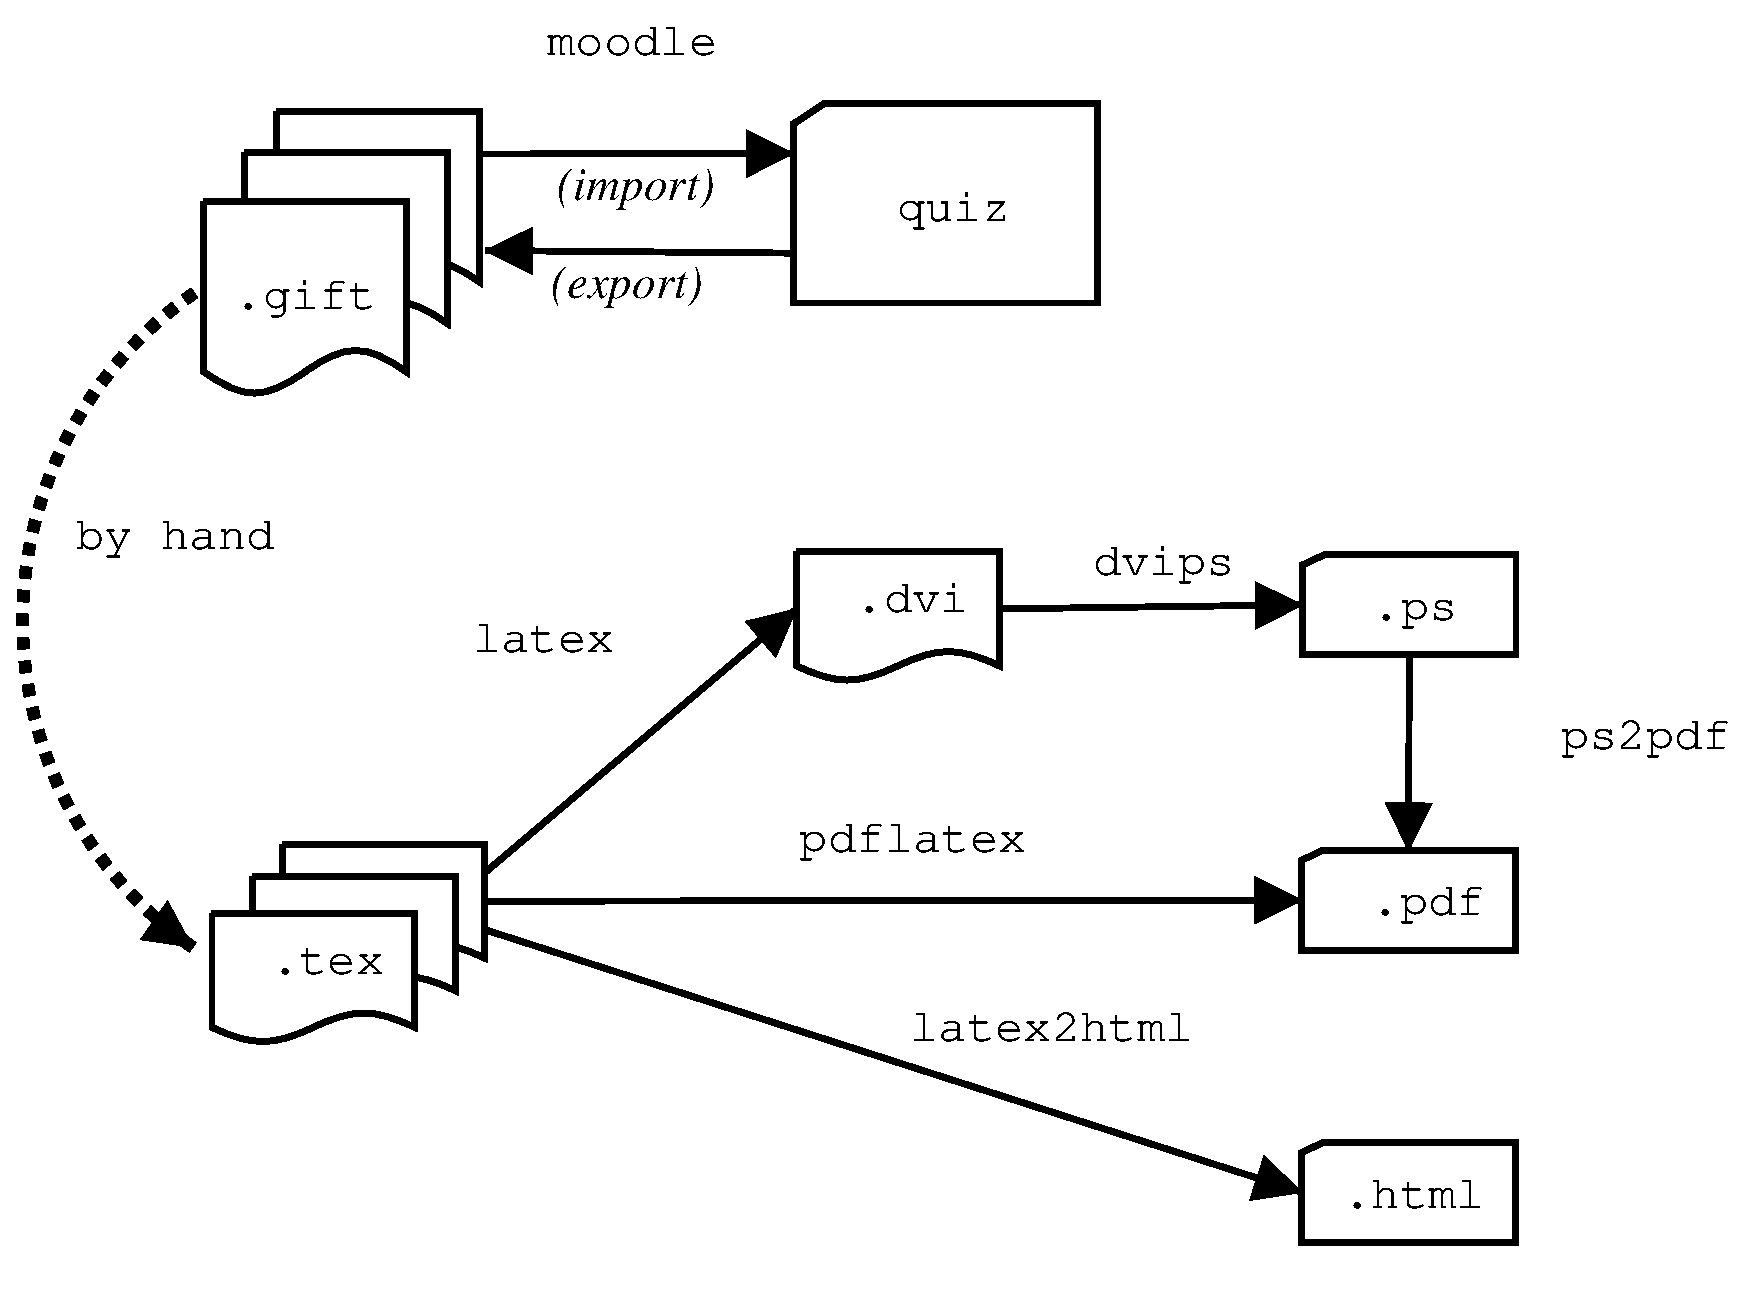
\includegraphics[scale=0.3]{methodology}
    \caption{Scheme of the methodology for the document generation}
    \label{fig:metogen}
  \end{center}
\end{figure}

%
Moodle has been adopted by our ``Escuela
T\'ecnica Superior de Ingenier\'{\i}a Inform\'atica de la Universidad de
La Laguna'', the place where we teach \cite{url:est} subjects
like Compilers, Programming, OOP, Parallel Programming, etc. 
Therefore, we had to migrate and integrate the existing material 
to the new platform.
The part requiring major effort was the 
preparation of questionnaires and problem sheets
(See Figure~\ref{fig:metogen}).
It was necessary to export, translate and import 
the interactive questionnaires 
to have both reactive and unreactive versions
of them.  

A warning about the use of electronic questionnaires.
Wh\-e\-n dealing with the evaluation of our students 
we usually differentiate between two kinds of evaluation:
\begin{itemize}
\item Additive Evaluation: The information is used to grade and credit the
student certificating the level of competentece reached.
\item Formative Evaluation: the information is used to guide and improve the
learning process
\end{itemize}
The most important attribute of the Formative Evaluation
is its capacity to provide \underline{timely information} even if not as accurately
as we can expect for Additive Evaluation.
It is for this purpose that the use of electronic questionnaires
and multiple-choice type exams is valuable. 

To better illustrate the methodology for the preparation of documents,
let us consider the make up of an exercise sheet for 
autoevaluation. 

%+++++++++++++++++++++++++++++++++++++++++++++++++++++++++++++++++++++++++++++
\subsection*{Step 1. Preparing the Quiz}

The easiest way to write a questionnaire is 
to take advantage of the 
Moodle interface for building questionnaires. 
That is straightforward to use, but,
depending on the circumstances, it can be unbearably 
slow. After filling the corresponding forms
you can export the questionnaire to \textsc{gift} format.

According to the Moodle manual, \textsc{gift} is the most comprehensive import / export
format available for importing quiz questions from/to a text file. 
It supports Multiple-Choice, True-False, Short Answer, Matching
and Numerical questions.  Various question-types can be mixed in a single text file,
and the format also supports line comments, question names, feedback for the student
and percentage-weight grades.

To export the questionnaire, select ``Questionnaire''.
Once in the edition window, choose the option ``Export questions to file''
. 
That will open a new window. 
Choose  the format and the name of the file.
By default the file is stored in the server inside the course subdirectory 
\verb|questionnaire|.


\begin{figure}[htb]
\mbox{}\hrulefill
\vspace{-.6em}
\begin{footnotesize}
\begin{verbatim}
 1 // question: 401  name: FIRST 
 2 ::FIRST::[html]Given a <i>grammar</i> 
 3 $$G\=(\Sigma,V,P,S)$$ and  a
 4 <i>production</i> $$A \rightarrow \alpha$$ 
 5 it holds that 
 6 $$FIRST(\alpha) \= \emptyset$$ implies 
 7 $$A$$ is annullable?{FALSE}
 8 
 9 // question: 402  name: accesing 
10 ::accesing::[html]A multidimensional array in C 
11 is simulated defining 1 dimensional arrays 
12 whose elements are arrays. To compute the 
13 relative position of one element  
14 $$a[i_1, i_2, ..., i_k]$$   
15 the following formula is applied:{
16  =$$(i_k + D_k(... (i_2 + i_1*D_2...))*size+ 
17   base-(L_k+D_k(... L_2+L_1*D_2...))*size$$
18  ~$$(i_k + D_k(...(i_3 + (i_2 + i_1*D_2)*D3)
19                ...)) * size + base$$
20  ~None of them
21 } \end{verbatim}
\end{footnotesize}
\vspace{-1.5em}
\hrulefill
\caption{GIFT file generated by Moodle from a Quiz}
\label{fig:ficherogift}
\end{figure}

Figure~\ref{fig:ficherogift} shows the result. 
We'll keep working with this example along this article.
%
Observe that questions are delimited by a double carriage-return.
%
The first question (lines 1-7) is an example of a \textsc{true-false} question.
%
Each question is divided into three sections:
%
The statement prefix,
the answer section bounded by the pair of non escaped
curly brackets and the statement postfix. 
%
Comments, like the one in line~1, start with two slashes and expand to the end of the line.
%
The prefix occupies lines from~2 to~7.  The text between pairs
of colons is the question identifier. Next, between brackets
comes the format used for this question. These two fields
are optional.
The source format in the example 
is \textsc{html} expanded with \TeX{}.
This is achieved through the \TeX{}
filter MimeTeX. 
%
The MimeTeX filter extends Moodle with 
the capacity of managing \TeX{} formulas
(\cite{url:forkosh, url:leiser}).
MimeTeX is always in math-like mode. 
Any text between \verb|$$| delimiters is interpreted by Moodle as a math formula 
and sent to the filter which renders the corresponding image.
%
%
It may optionally start with the name of the question enclosed by a pair of colons and the 
format (\textsc{html}, \textsc{plain}, etc.). 
%
When the \TeX{} filter is installed the text is a combination of  \textsc{html}
and 
\LaTeX{}. 
%
The correct answer appears between braces in line~7. 
\LaTeX{} formulas can also be used in this section.
%
Lines~9-21 present a \textsc{multiple-option} question.
%
The correct answer is prefixed by the symbol  ``\verb|=|'' while wrong answers have 
a ``\verb|~|'' at the beginning. 


\begin{figure}[htb]
\mbox{}\hrulefill
\vspace{-.6em}
\begin{footnotesize}
\begin{verbatim}
 Given a grammar
 $$G =(\Sigma,V,P,S)$$ 
 and  a production 
 $$A \rightarrow \alpha$$ 
 does $$FIRST(\alpha) = \emptyset$$ 
 implies $$A$$ is annullable?{FALSE}
 
 A multidimensional array in C 
 is simulated defining 1-dimensional arrays 
 whose elements are arrays. To compute the 
 relative position of one element  
     $$a[i_1, i_2, ..., i_k]$$   
 the following formula is applied:
 {
  =$$(i_k + D_k(... (i_2 + i_1*D_2...))*size+ 
   base-(L_k+D_k(... L_2+L_1*D_2...))*size$$
  ~$$(i_k + D_k(...(i_3 + (i_2 + i_1*D_2)*D3)
                ...)) * size + base$$
  ~None of them
 } \end{verbatim}
\end{footnotesize}
\vspace{-1.5em}
\hrulefill
\caption{GIFT file. ``Human Informal Style'' }
\label{fig:ficherogifthuman}
\end{figure}

An alternative and faster way 
to the Moodle interface is to directly write the \textsc{gift}
with your document 
favourite editor.
This approach makes easier the recycling of existing \LaTeX{}
and \textsc{HTML} material and may be automatized through somewhat 
ad-hoc scripts. It also allows for a more 
``relaxed'' and human readable \textsc{GIFT} files.


\begin{figure}[!ht]
  \begin{center}
    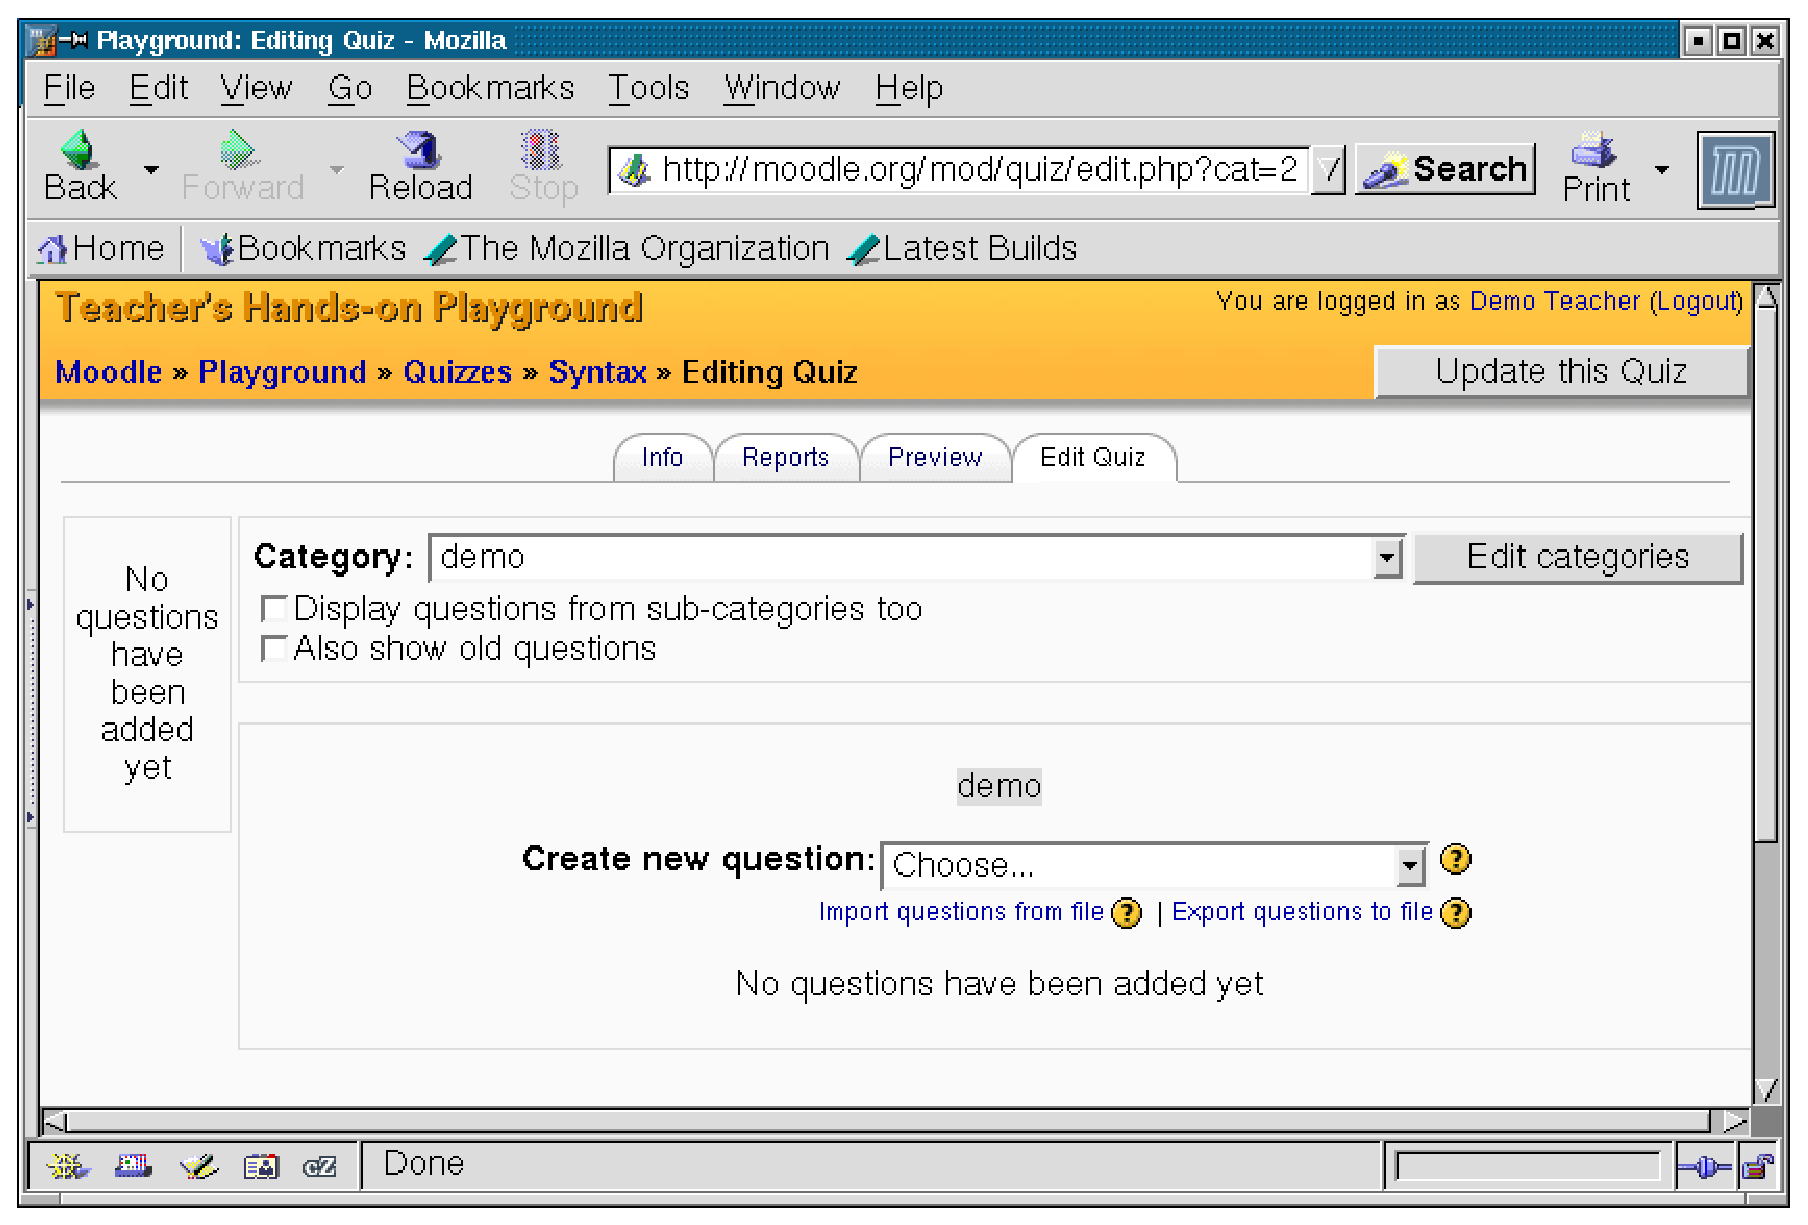
\includegraphics[scale=0.3]{EditingQuiz}
  \end{center}
\caption{Editing a Quiz}
\label{fig:quiz:1}
\end{figure}

\begin{figure}[!ht]
  \begin{center}
    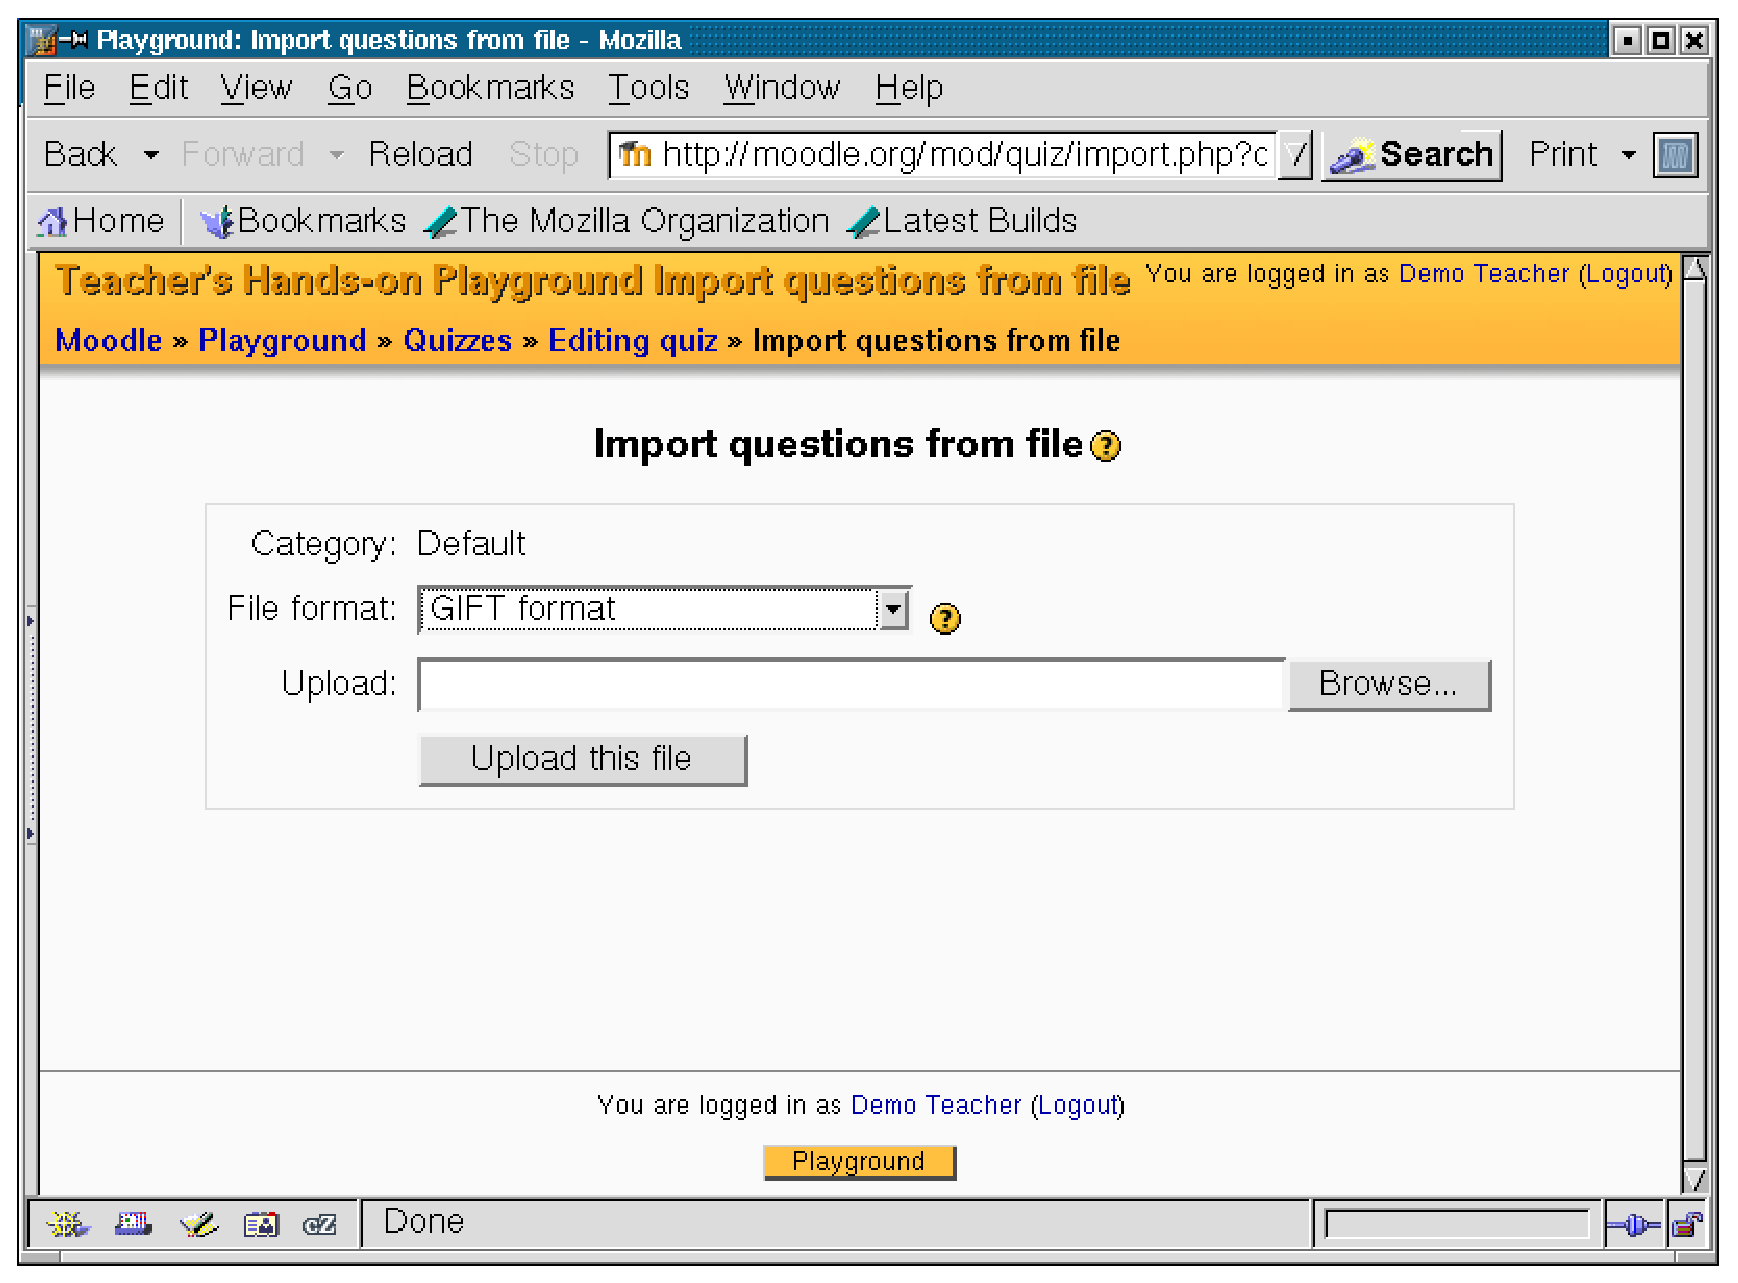
\includegraphics[scale=0.3]{importFromfile}
  \end{center}
\caption{Loading the file}
\label{fig:quiz:2}
\end{figure}

\begin{figure}[!ht]
  \begin{center}
    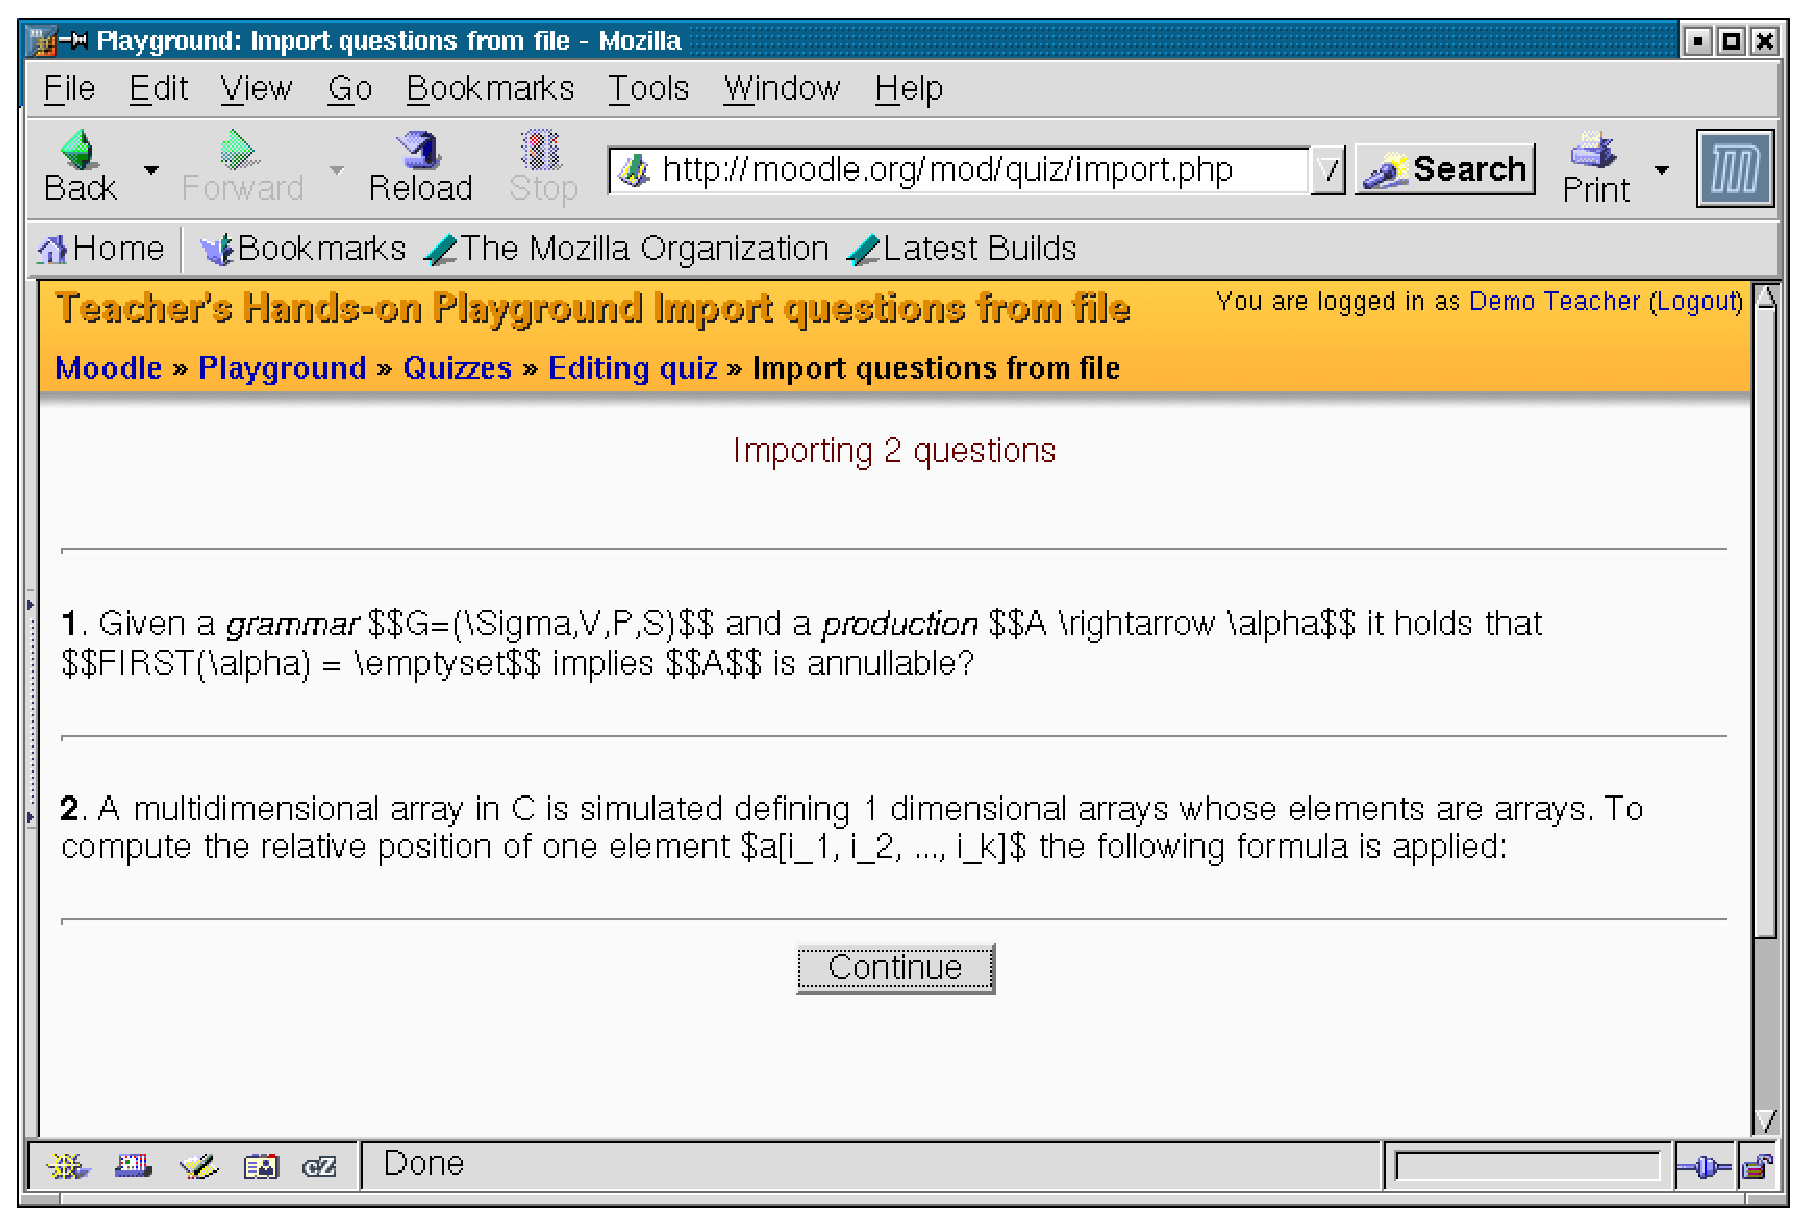
\includegraphics[scale=0.3]{importing2questions}
  \end{center}
\caption{A GIFT file has been uploaded}
\label{fig:quiz:3}
\end{figure}

Figure \ref{fig:ficherogifthuman} shows  a typical
``human edited'' version
of the example in Figure~\ref{fig:ficherogift}. 
The file appears less cluttered among other reasons because
\textsc{gift} metasymbols (like \verb|=|, \verb|~|, 
\verb|{|,\verb|}|, etc.) aren't escaped.
The escape is done through a utility script acompanying
the software presented in Section 
\ref{section:pro}.

If we choose the last option, we have to import/upload the
\textsc{gift}  file to the Moodle site.
This also gives a path 
to migrate the exercises to another courses or
another Moodle installation.
To import a quiz, edit an activity of type ``questionnaire''
and once in the edition window (Figure~\ref{fig:quiz:1}) 
select the option ``Import questions from file''.
A window like the one in Figure~\ref{fig:quiz:2} is open. 
From there we can proceed to locate the file and to upload it.
The result of a succesful upload is displayed in Figure~\ref{fig:quiz:3}.

%+++++++++++++++++++++++++++++++++++++++++++++++++++++++++++++++++++++++++++++
\subsection*{Step 2. Preparing the Material in \LaTeX{}}

To obtain equivalent high-quality non-reactive formats
we translate the \textsc{gift} file into a new \LaTeX{}
file.
Figure~\ref{fig:autoevaluacionLaTeX} shows a human-made
direct translation  to \LaTeX{} where two
nested enumerate environments have been used.
From the \LaTeX{} version we can easily obtain
postcript using \texttt{dvips}, 
\textsc{pdf} using \texttt{pspdf} or \texttt{pdflatex}
and \textsc{html} 
using \texttt{latex2html}.
Though they were actually obtained using the tool to be described
next in Section
\ref{section:pro}, Figures \ref{fig:ps} and
\ref{fig:html}
give you an idea of the final 
appearance.

\begin{figure}[htb]
\mbox{}\hrulefill
\vspace{-.6em}
\begin{footnotesize}
\begin{verbatim}
 1 \begin{enumerate}
 2 \item
 3   Given a \emph{grammar} $G=(\Sigma,V,P,S)$ and
 4   a \emph{production} $A \rightarrow \alpha$ it
 5   holds that $FIRST(\alpha) = \emptyset$
 6   implies \emph{A} is annullable?
 7   \begin{enumerate}
 8     \item
 9       True
10     \item
11       False
12   \end{enumerate}
13
14 \item
15   A multidimensional array in C is simulated
16   defining 1 dimensional arrays whose elements
17   are arrays. To compute the relative position
18   of one element $a[i_1, i_2, ..., i_k]$ the
19   following formula is applied:
20   \begin{enumerate}
21     \item
22       $(i_k + D_k(... (i_2 + i_1*D_2...))*size+
23       base-(L_k+D_k(... L_2+L_1*D_2...))*size$
24     \item
25       $(i_k + D_k(...(i_3 + (i_2 +
26              i_1*D_2)*D3)...)) * size + base$
27     \item
28     None of them
29   \end{enumerate}
30 \end{enumerate} \end{verbatim}
\end{footnotesize}
\vspace{-1.5em}
\hrulefill
\caption{Quiz exercises in \LaTeX{} format}
\label{fig:autoevaluacionLaTeX}
\end{figure}

\begin{figure}[hbt]
  \begin{center}
    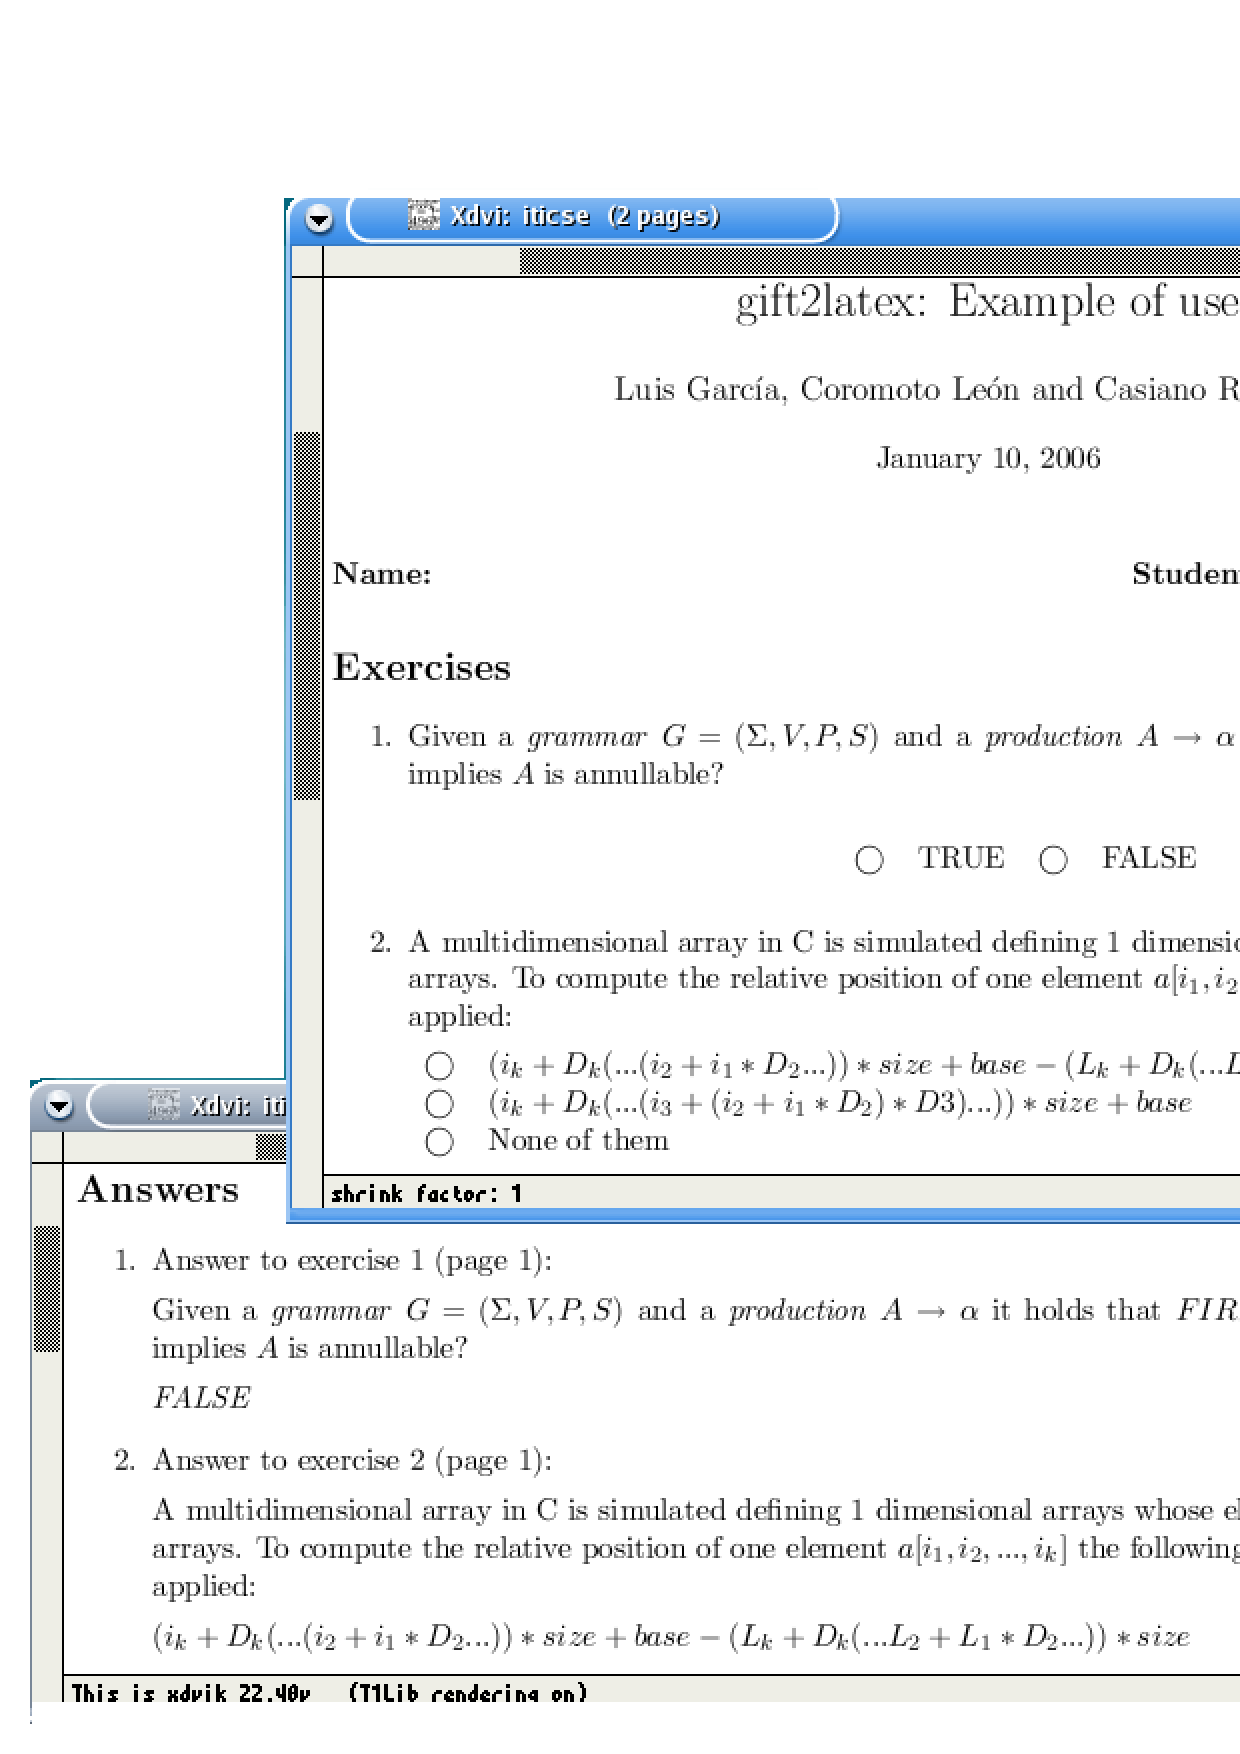
\includegraphics[scale=0.3]{gift2ps}
  \end{center}
\caption{Postscript generated from \LaTeX{}}
\label{fig:ps}
\end{figure}



\begin{figure}[hbt]
  \begin{center}
    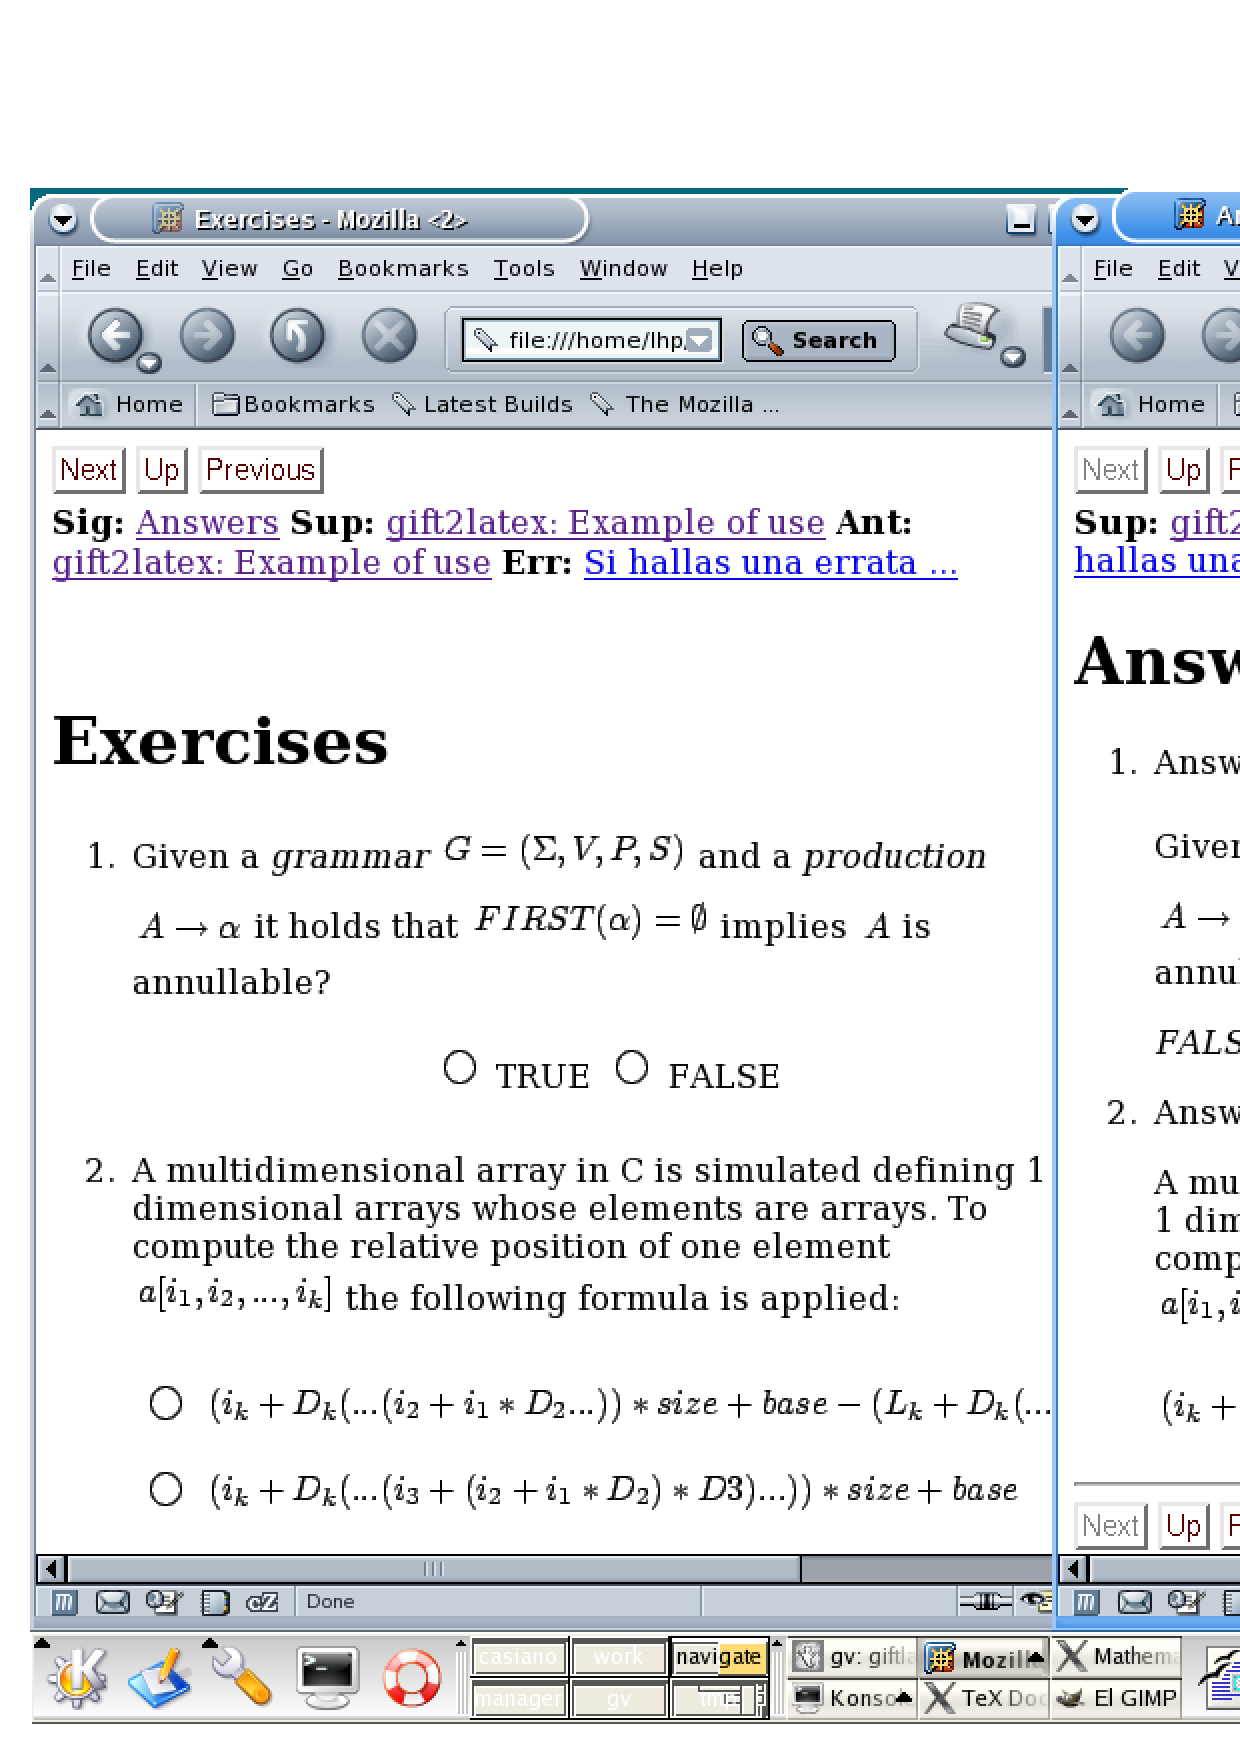
\includegraphics[scale=0.3]{gift2html}
  \end{center}
\caption{HTML generated by \LaTeX2HTML{}}
\label{fig:html}
\end{figure}

%--------------------------------------------------------------------------------------
\section{Automatic Solution}
\label{section:pro}
%\input{automatica}

\begin{figure}[!ht]
  \begin{center}
    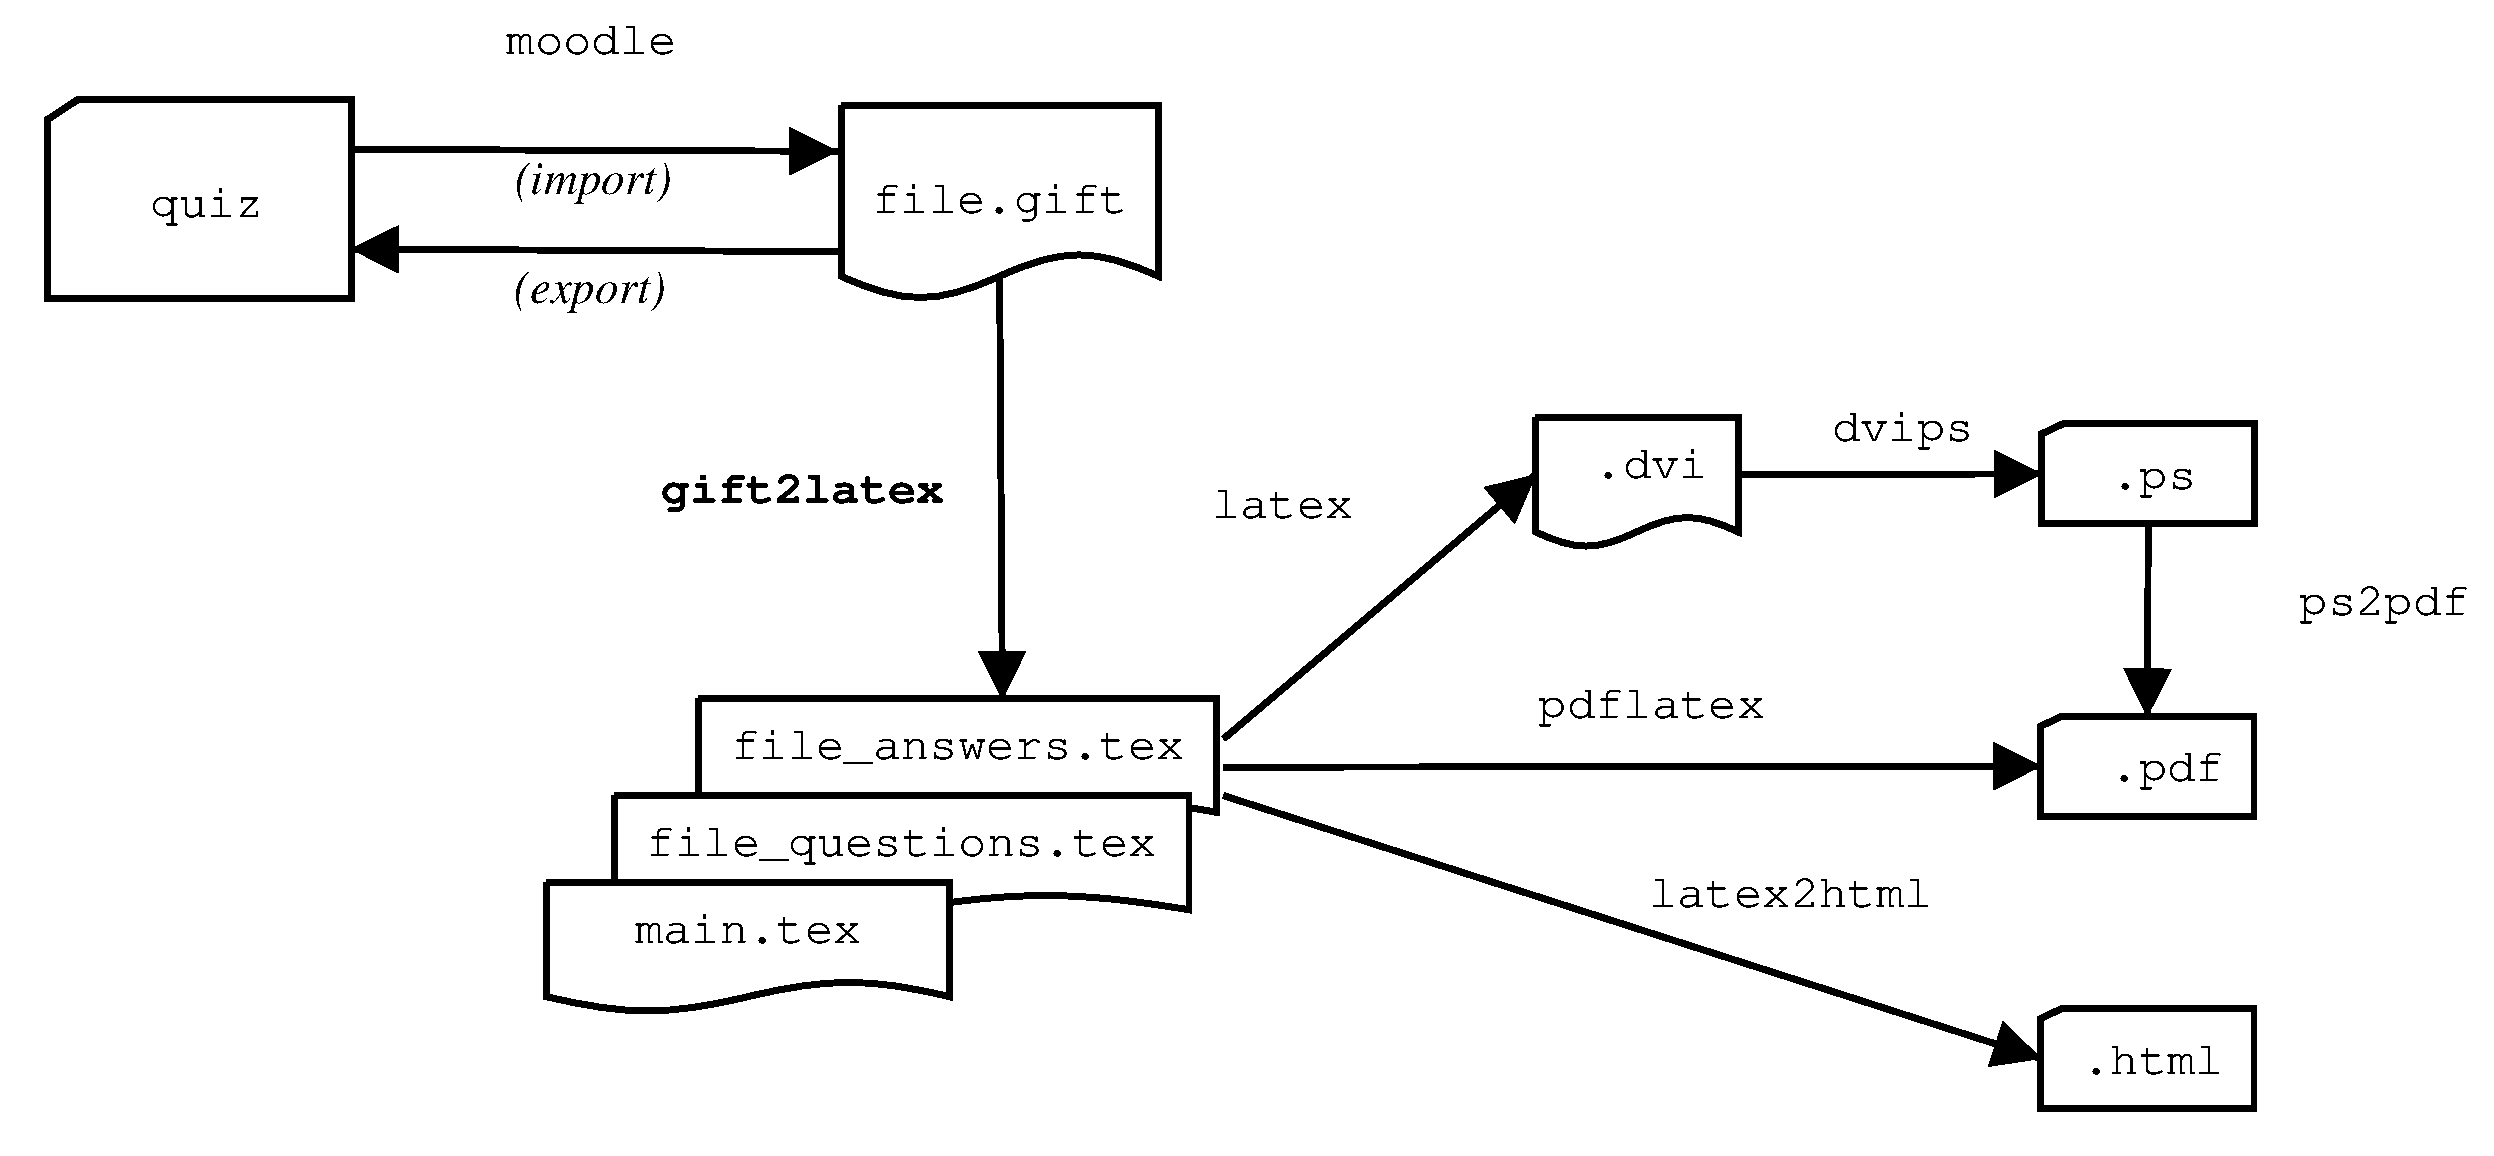
\includegraphics[scale=0.3]{automatic}
    \caption{Scheme using automatic translation}
    \label{fig:automatic}
  \end{center}
\end{figure}

Starting from an interactive quiz and following the steps described in the 
former section there is always a mean to produce a file in \textsc{gift}
format describing the questions.
%
The translation is made by a Perl~\cite{Wal:91} program named \texttt{gift2\-latex}.  
%
Figure~\ref{fig:automatic} outlines the process.
%
The first step to obtain one of the unreactive formats from the quiz 
(\textsc{pdf}, Postcript, etc.) is to export the quiz to \textsc{gift} format.  
%
As is described in the previous section, this transformation is bidirectional, 
that is, Moodle allows both import and export operations on \textsc{gift} files.
%
From this source, the script \texttt{gift2latex} produces two \LaTeX{} files; 
Each one contains a \LaTeX{} section. The
first one describes the questions.  The second (referenced by the former)
describes the answers. 
%
However, depending on the execution options the output can be a standalone full latex 
document or the two files describing the questions and answers, 
to be included inside a main document. 

\begin{figure}[hbt]
\mbox{}\hrulefill
\vspace{-.6em}
\begin{footnotesize}
\begin{verbatim}
 1 \item
 2 \label{question:syntax1}
 3 Given a \emph{grammar}
 4  $G=(\Sigma,V,P,S)$ and a \emph{production}
 5  $A \rightarrow \alpha$ it holds that 
 6  $FIRST(\alpha) = \emptyset$ 
 7  implies $A$ is annullable?
 8 
 9 \begin{center}
10 \begin{tabular}{llll}
11 $\bigcirc$ & TRUE & $\bigcirc$ & FALSE
12 \end{tabular}
13 
14 \noindent 
15 \end{center} \end{verbatim}
\end{footnotesize}
\vspace{-1.5em}
\hrulefill
\caption{Excerpt of the \LaTeX{} file for the question section}
\label{fig:questions}
\end{figure}

\begin{figure}[hbt]
\mbox{}\hrulefill
\vspace{-.6em}
\begin{footnotesize}
\begin{verbatim}
 1 \item Answer to exercise
 2 \label{answer:syntax1}
 3 \ref{question:syntax1}
 4 (page
 5 \pageref{question:syntax1}):
 6 
 7 \noindent Given a \emph{grammar}
 8  $G=(\Sigma,V,P,S)$ and a \emph{production}
 9  $A \rightarrow \alpha$ it holds that
10  $FIRST(\alpha) = \emptyset$ 
11  implies $A$ is annullable?
12 
13 \emph{FALSE}
\end{verbatim}
\end{footnotesize}
\vspace{-1.5em}
\hrulefill
\caption{Excerpt of the \LaTeX{} file for the answer section}
\label{fig:answers}
\end{figure}

Let us assume the quiz shown in Figure~\ref{fig:ficherogift} is stored in 
a file named \verb|exercises.| \verb|gift|.
%
Figures \ref{fig:questions} and \ref{fig:answers} show fragments of the ouputs 
obtained when executing the command line:

\begin{center}
\verb|$ gift2latex exercises.gift| 
\end{center}

\noindent the two generated files (named exercises\_questions.tex and
exercises\_answers.tex) can then be embeded inside a main document
using the \LaTeX{} \verb|\input| command.

Observe that the \LaTeX{} code in Figure~\ref{fig:questions}
is more sophisticated than the one
in Figure~\ref{fig:autoevaluacionLaTeX}. 
Links between each pair of question-answer 
items are generated.


\begin{figure}[hbt]
\mbox{}\hrulefill
\vspace{-.6em}
\begin{footnotesize}
\begin{verbatim}
 1 %<$separator%>
 2 \label{question:%<$label%>}
 3 %<$prefix%>
 4 
 5 \begin{center}
 6 \begin{tabular}{llll}
 7 $\bigcirc$ & TRUE & $\bigcirc$ & FALSE
 8 \end{tabular}
 9 
10 \noindent %<$sufix%>
11 \end{center} \end{verbatim}
\end{footnotesize}
\vspace{-1.5em}
\hrulefill
\caption{Excerpt of the template for TRUE-FALSE}
\label{fig:truefalsetemplate}
\end{figure}

Figures~\ref{fig:ps} and~\ref{fig:html} showed a 
visual sample of the result of compiling with \LaTeX{} 
and \LaTeX2HTML{} the \LaTeX{} files generated by \textsc{gift2latex}.
%
The \textsc{html} version is navigable: Clicking the question buttons (left figure)
takes you to the corresponding item inside the Answer section (right).


Teachers can change the style of the output modifying the 
coresponding style files, usually found
in the \verb|etc| distribution directory.
%
There are a couple of style files per type of question.
They control
the output aspects for the question and answer sections. 
The syntax to describe a style 
is a mixture of \LaTeX{} and Perl.
%
Figure~\ref{fig:truefalsetemplate} presents a fragment of 
a translation template or style file for \textsc{true-false}
questions.
Chunks of text between the \verb|%<| and \verb|%>| correspond to the variable part
(Perl code) inside the fix \LaTeX{} structure.

%-------------------------------------------------------------------------------

\section{Conclusions}
\label{section:conclusiones}
%\input{conclusions}

This work discusses the problem of integrating Moodle and LaTeX{} documents
proposes a methodology to solve it and presents a tool to assist 
in the translation of questionnaires.
The steps to produce the materials are:
\begin{enumerate}
\item 
Write a questionnaire 
taking advantage of the 
Moodle interface for building questionnaires.
\item After filling the corresponding forms,
export the questionnaire to \textsc{gift} format.
\item
Run the script \texttt{gift2latex} on this file: it produces two \LaTeX{} files; 
One describes the questions, the other the answers. 
%
\item
Finally, include these files in the main latex document. 
\end{enumerate}
Alternatively, since GIFT is more human friendly than other formats as XML, 
the lecturer can omit steps 1 and 2 and directly edit the questionnaire in GIFT formatusing her favourite editor.

The tool is currently a functional prototype and we
expect it will be soon delivered in CPAN 
\cite{url:cpan}. 
A version of the front-end \textsc{gift} parser is already there \cite{url:gift2latex}.



%%%%%%%%%%%%%%%%%%%%%%%%%%%%%%%%%%%%%%%%%%%%%%%%%%%%%%%%%%%%%%%%%%%%%%%%%%%%%%%%%%%%%%%%
\section{Acknowledgments}

This work has been supported by the {\sc ec (feder)} and by the Spanish Ministry of 
Education inside the `Plan Nacional de {\sc i+d+i}' with contract number 
{\sc tic2005-08818-c04-04}.

%%%%%%%%%%%%%%%%%%%%%%%%%%%%%%%%%%%%%%%%%%%%%%%%%%%%%%%%%%%%%%%%%%%%%%%%%%%%%%%%%%%%%%%%
%\bibliographystyle{abbrv}
%\bibliographystyle{alpha}
\bibliographystyle{unsrt}
\bibliography{giftlatex}  

\end{document}
